\documentclass[a4paper,ngerman,12pt]{zirkelblatt1415}

\usepackage[utf8]{inputenc}

\usepackage[ngerman]{babel}

\usepackage{amsmath,amsthm,amssymb,stmaryrd,color,graphicx}
\usepackage{setspace,icomma}
\usepackage{bussproofs}
\usepackage{array}
\usepackage{comment}
\usepackage{graphicx}
\usepackage[protrusion=true,expansion=true]{microtype}

\usepackage{lmodern}

\usepackage{hyperref}

\setlength\parskip{\medskipamount}
\setlength\parindent{0pt}

 \theoremstyle{definition}
 \newtheorem{definition}{Definition}
% \newtheorem{axiom}[defn]{Axiom}
% \newtheorem{bsp}[defn]{Beispiel}

% \theoremstyle{plain}
% \newtheorem{prop}[defn]{Proposition}
% \newtheorem{motto}[defn]{Motto}
% \newtheorem{wunder}[defn]{Wunder}
% \newtheorem{ueberlegung}[defn]{Überlegung}
% \newtheorem{lemma}[defn]{Lemma}
% \newtheorem{kor}[defn]{Korollar}
% \newtheorem{hilfsaussage}[defn]{Hilfsaussage}
 \newtheorem{satz}[definition]{Satz}
% \newtheorem{frage}[defn]{Fragestellung}
 \newtheorem{beispiel}[definition]{Beispiel}
% \newtheorem{problem}[defn]{Problemstellung}


\theoremstyle{remark}
\newtheorem{bem}[definition]{Bemerkung}
% \newtheorem{aufg}[defn]{Aufgabe}

%\newlength{\aufgabenskip}
%\setlength{\aufgabenskip}{1.0em}
%\newcounter{aufgabennummer}
%\newenvironment{aufgabe}[1]{
%  \addtocounter{aufgabennummer}{1}
%  \textbf{Aufgabe \theaufgabennummer.} \emph{#1} \par
%}{\vspace{\aufgabenskip}}

% \clubpenalty=10000
% \widowpenalty=10000
% \displaywidowpenalty=10000

 \setlength\unitlength{1cm}

% \RequirePackage{geometry}
% \geometry{textwidth=16.0cm,textheight=24.5cm,footskip=1.5cm}
% \DeclareGraphicsExtensions{.pdf,.png,.jpg}

\usepackage[bottom=4cm]{geometry}
\usepackage{textcomp}

\newcommand{\RR}{\mathbb{R}}
\newcommand{\CC}{\mathbb{C}}
\newcommand{\ZZ}{\mathbb{Z}}
\renewcommand{\NN}{\mathbb{N}}
\newcommand{\QQ}{\mathbb{Q}}
\newcommand{\lra}{\longrightarrow}
\newcommand{\id}{\text{id}}
\newcommand{\ol}[1]{\overline{#1}}

\begin{document}

\begin{picture}(0,0)
  \put(0,-0.5){%
    
\includegraphics[scale=0.1]{bilder/logo-ifm}
  }
  \put(14.0,-3.5){%
    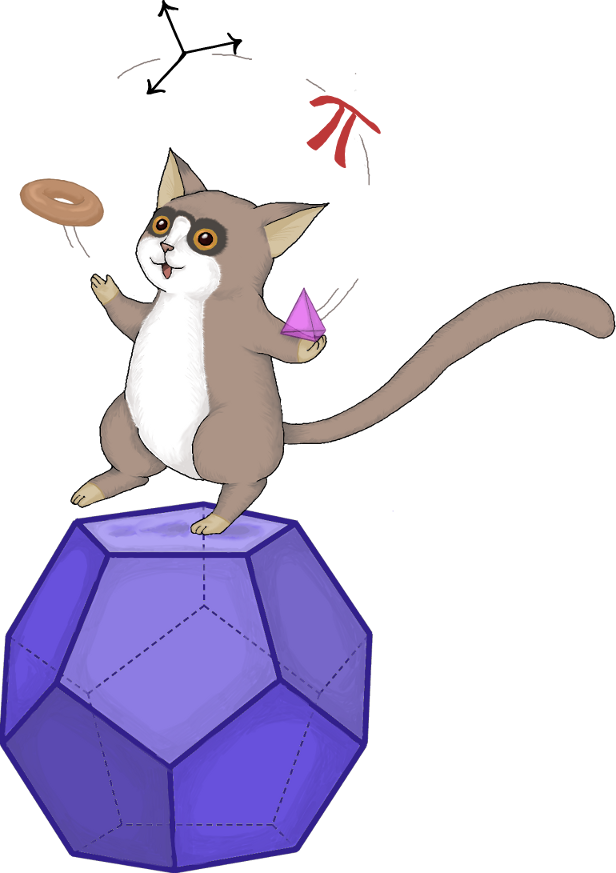
\includegraphics[scale=0.17]{bilder/cover}
  }
\end{picture} 

\vspace{6em}


\begin{center}\Large{Vierter Korrespondenzbrief vom \today}\end{center}

\begin{center}\Large{Iterierte Funktionensysteme: Kochkurve und Zeltabbildung}\end{center}

In diesem Brief geht es um Funktionen und deren wiederholtes Anwenden. In der Schule habt ihr vielleicht bereits Funktionen\footnote{Funktionen werden auch manchmal Abbildungen genannt. Dieser Begriff ist sehr allgemein und Funktionen bezeichnen meist nur Abbildungen, die eine Zahl nehmen und daraus eine neue Zahl machen.} kennengelernt, hier wollen wir zunächst etwas allgemeiner darüber sprechen und dann Beispiele anschauen, welche "`zeitliche Veränderungen von Zuständen"' beschreiben sollen und so ein "`einfaches"'\footnote{Wie wir sehen werden, sind sie überhaupt nicht einfach.} Beispiel für sogenannte \emph{dynamische Systeme} darstellen.

\section{Grundlagen}

Bevor wir über Funktionen reden, wollen wir einige Grundlagen besprechen.
\begin{definition}
Eine \emph{Funktion} $f$ ist eine Abbildungsvorschrift von einer Menge $A$ in eine Menge $B$, kurz $f:A\rightarrow B$, die jedem Element $x$ aus $A$ \emph{genau ein} Element $f(x)$ aus $B$ zuordnet.
Man schreibt auch:
\[
f: x \mapsto f(x).
\]
$A$ heisst \emph{Definitionsbereich} und $B$ \emph{Bildbereich}.
\end{definition}

\begin{beispiel}
\begin{enumerate}
\item Die Funktion $f$, die zu jeder gegebenen reellen Zahl Eins dazuaddiert ist gegeben durch $f:\RR\lra\RR$ mit $f(x)=x+1$.
\item Die Abbildung "`Verdoppeln"' $g$ auf den reelen Zahlen $\mathbb{R}$ kann geschrieben werden als $g:\mathbb{R}\rightarrow\mathbb{R}$ mit
\[
g : x \mapsto 2x
\]
oder kürzer als $g(x)=2x$.
\item Das Runden einer reellen Zahl kann als eine Funktion $h$ aufgefaßt, $h:\mathbb{R}\longrightarrow\mathbb{Z}$, in die ganzen Zahlen. So gilt zum Beispiel $h(0,321)=0$, $h(0,5)=1$ (nach üblicher Konvention) und $h(2)=2$.
\end{enumerate}
\end{beispiel}

Auf jeder Menge $A$ gibt es eine besondere Abbildung, und zwar die Identität $\text{id}_A$, die jedes Element auf sich selbst abbildet. Zum Beispiel gilt für $\id_{\RR}\RR\lra\RR$, dass $\id_{RR}(3,7)=3,7$ ist. Die Identitätsabbildung darf man aber nicht verwechseln mit einer \emph{konstanten Abbildung} $\text{const}_{c}:\RR\lra\RR$, wobei $c\in\RR$ eine beliebige gewählte (aber jetzt feste) reelle Zahl ist. Diese Funktion ist definiert mittels $\text{const}_c(x)=c$, das heißt, sie ordnet \emph{jeder} reellen Zahl die gleiche Zahl zu, nämlich $c$.


Man kann eine Funktion $f$ natürlich dadurch definieren, dass man für jedes Element $x$ das Bildelement $f(x)$ angibt, was aber für sehr große Mengen\footnote{Insbesondere gilt dies für unendliche Mengen wie die üblichen Zahlenbereiche $\NN$, $\QQ$, $\ZZ$, $\RR$ und $\CC$.} etwas kompliziert ist. Einfacher ist es, wenn man eine "`Formel"' angibt, welche den Funktionswert durch das Argument ausdrückt. Manchmal findet man aber keine Vorschrift, die für alle Elemente vom Definitionsbereich gilt. Betrachte als Beispiel die Betragsfunktion $b:\mathbb{R} \mapsto \mathbb{R}^+_0$, die jeder reelen Zahl eine nichtnegative Zahl zuordnet: Jede Zahl $x$, die größer oder gleich Null ist, wird auf sich selbst abgebildet. Eine negative Zahl $x$ wird auf $-x$ abgebildet. Man kann also kurz schreiben
\[ b(x) =\begin{cases} 
      x & x\geq 0 \\
      -x & x < 0
   \end{cases}.
\]
Für den Betrag einer Zahl $x$ schreibt man üblicherweise $|x|$, also gilt $b(x)=|x|$. Solche Fallunterscheidungen liest man wie folgt: Wenn das Argument $x$ größer oder gleich Null ist, so nimmt $b$ den Wert an, welcher in der Zeile für diesen Fall steht, hier also die obere Zeile, wo $b(x)=x$ notiert ist. Falls aber $x<0$ gilt, so sind wir auf der unteren Zeile, wo $b(x)=-x$ steht.

Als weiteres Beispiel können wir einen Funktion $r$ definieren, die jeder natürlichen Zahl ihren Rest bei der Division durch $2$ zuordnet: $r:\mathbb{N}_0 \longrightarrow \{0\text{, }1\}$ mit
\[ r(a) = 
\begin{cases}
0 & 2\mid a \\
1 & 2\nmid a.
\end{cases}
\]
Hier bedeutet $2 \mid a$, dass $2$ ein Teiler von $a$ ist, also $a$ gerade ist, und $2\nmid a$ genau das Gegenteil. Wir sagen, dass es sich in den Fällen von $b$ und $f$ um \emph{abschnittsweise definierte Funktionen} handelt.

Wenn wir eine Funktion $f:A\lra B$ gegeben haben, wissen wir, was mit dem Definitionsbereich $A$ unter $f$ geschieht und welche Elemente vom Bildbereich $B$ angenommen werden. Was ist aber mit Teilmengen dieser Mengen? Dazu gibt es den Begriff des Bilds und des Urbilds.

\begin{definition}
Sei $f:A\longrightarrow B$ eine Abbildung und $A_0\subset A$ eine Teilmenge von $A$. Dann bezeichnen wir mit dem \emph{Bild von} $A$, kurz $f(A_0)$, die Menge aller Elemente 
$y$ von $B$, so dass es ein $x\in A_0$ gibt mit $f(x)=y$ oder in Formelsprache
$f(A_0) = \{y\in B\,|\,\text{Es gibt ein } x\in A_0 \text{ mit } f(x) =y\}.$ 
\end{definition}

\begin{beispiel}
  Beispiel zu Bildern von Abbildungen mit Bild.
\end{beispiel}

\begin{aufgabe}{Bilder von Abbildungen}
  Aufgabe zu Bildern von Abbildungen.
\end{aufgabe}

\begin{definition}
Sei $f:A\longrightarrow B$ eine Abbildung und $B_0\subset B$ Teilmenge von $B$. Dann bezeichnen wir mit dem \emph{Urbild von} $B_0$, kurz $f^{-1}(B_0)$, die Menge aller Elemente 
$x$ von $A$, so dass es ein $y\in B_0$ gibt, mit $f(x)=y$ oder in Formelsprache
$f^{-1}(B_0) = \{x\in A\,|\,\text{Es gibt ein } y\in B_0 \text{ mit } f(x) =y\}.$ 
\end{definition}

\begin{beispiel}
\begin{enumerate}
\item
\item Betrachte die Betragsfunktion $b$ von vorhin. Dann haben wir
\begin{align*}
b([-1,1]) &=  [0,1] \\
b^{-1}([-1,2]) &= [-2,2]\\
b^{-1}((-\infty, 0)) &= \emptyset\footnotemark.
\end{align*}
\footnotetext{Das Zeichen $\emptyset$ bezeichnet die sogennante \emph{leere Menge}, also die Menge, die kein Element beinhaltet (also auch nicht die Null).}
\item
\end{enumerate}
\end{beispiel}

\begin{aufgabe}{Urbilder von Abbildungen}
  Aufgabe zu Urbildern von Abbildungen.
\end{aufgabe}

\begin{aufgabe}{Leider ist die Welt manchmal nicht ganz einfach.}
Sei eine Abbildung $f:A\longrightarrow B$ und  $A_0\subset A$ und $B_0\subset B$. Im Allgemeinen gilt 
\begin{align*}
f^{-1}\left(f\left(A_0\right)\right) &\neq A_0,\\
f\left(f^{-1}\left(B_0\right)\right) &\neq B_0.
\end{align*}
Das heißt, dass im Allgemeinen das Bild des Urbildes einer Menge nicht die Menge selbst und das Urbild des Bildes einer Menge nicht die Menge selbst ist. Finde Beispiele für beide Aussagen. \emph{Hinweis: Die Betragsfunktion bietet sich dafür an.}
\end{aufgabe}

Wenn wir zwei Abbildungen $f$ und $g$ haben, können wir beide unter Voraussetzungen \emph{miteinander verknüpfen} und so eine neue Funktion erhalten.
\begin{definition}
Seien $f: A\longrightarrow B$ und $g: B\longrightarrow C$ zwei Abbildungen. Dann ist die Verknüpfung $g\circ f$ (ausgesprochen "`$g$ nach $f$"') eine Abbildung von $A$ nach $C$, die definiert ist als
\[
g\circ f: x \mapsto g\left(f(x)\right)
\]
oder anders geschrieben
\begin{equation*}
  g\circ f(x)=g(f(x)),
\end{equation*}
das heißt, zuerst wendet man $f$ an und danach $g$ auf das Ergebnis von $f$.
\end{definition}

\begin{bem}
  Beachte, dass die Reihenfolge der Schreibweise komisch ist: $g\circ f$ bedeutet, dass $f$ zuerst angewendet wird und nicht $g$. Das verknüpfte Abbildung nennt man auch manchmal die \emph{Komposition}.
\end{bem}

\begin{beispiel}
Sei $f:x\mapsto 2x$ und $b$ unsere Betragsfunktion. Dann ist
\[
b\circ f: x\mapsto |2x|.
\]
\end{beispiel}

\begin{aufgabe}{Vertauschen von Kompositionen}
In diesem Fall gilt $b\circ f = f \circ b$. Im allgemeinen, selbst wenn $f:A\mapsto A$ und $g:A\mapsto A$, haben wir
\[
f\circ g \neq g \circ f.
\]
Finde zwei Funktionen $f$ und $g$, so dass $f\circ g$ und $g\circ f$ beide existieren, die beiden jedoch unterschiedlich sind. 
\end{aufgabe}

Eine interessante Frage ist, ob man eine gegebene Abbildung "`umkehren"' kann.
\begin{definition}
Sei $f:A\longrightarrow B$. Eine Abbildung $f^{-1}:B\longrightarrow A$ heißt \emph{Umkehrabbildung} von $f$, wenn gilt:
\begin{align*}
f&\circ f^{-1} = \text{id}_B\\
f^{-1}&\circ f = \text{id}_A.
\end{align*}
\end{definition}

\begin{aufgabe}{Endliche Mengen und Abbildungen}
Seien $A$ und $B$ endliche Mengen und $f:A\longrightarrow B$ eine Abbildung zwischen diesen. Beweise die folgende Aussage:

Wenn $A$ und $B$ unterschiedlich viele Elemente haben, kann es keine Umkehrabbildung $f^{-1}$ zu $f$ geben.

Tipp: Behandle die beiden Fälle
\begin{enumerate}
\item $A$ hat mehr Elemente als $B$
\item $B$ hat mehr Elemente als $A$
\end{enumerate}
\end{aufgabe}

% \begin{aufgabe}
% Beweise die folgende Aussage: 

% Erfüllt die Funktion $f:A\longrightarrow B$ die beiden Eigenschaften:
% \begin{itemize}
% \item $f$ ist injektiv: Es gibt keine zwei verschiedenen Elemente $x_1$ und $x_2$ mit $f(x_1)=f(x_2)$.
% \item $f$ ist surjektiv: Jedes Element $y$ von $B$ ist Bild eines Element von $A$.
% \end{itemize}
% \end{aufgabe}

\section{Iterierte Funktionsysteme}
Haben wir eine Funktion $f:A\longrightarrow A$ von einer Menge in sicher selber, können wir betrachten, was passiert, wenn wir die Abbildung immer wieder mit sich selbst Verknüpfen. Dies bezeichnen wir als iteriertes\footnote{Itereren bedeutet einfach Wiederholen} Funktionsystem $f$ auf $A$.
\begin{beispiel}
Wir haben die Menge $A=\{1,2,3,4 \}$. Betrachten wir die Funktion
\[
f(x)=\begin{cases}
2 & x=2 \\
4 & x\in\{1,3\} \\
3 & x=4.
\end{cases}
\]
Das wird unsere Standardbeispiel für den Rest dieses Abschnitts. 
\end{beispiel}
Da es sehr mühsam ist, mit $\circ$ die Verknüpfung zu schreiben, gibt es eine verkürzende Schriebweise
\begin{definition}
\begin{align*}
f^n &= \underbrace{f \circ f \circ f \circ \ldots \circ f}_{\text{n-mal}}\\
f^0 &= id|_A.
\end{align*} 
\end{definition}
Was bei einem iterierten Funktionensystem vorallem interessiert, ist, wie sich ein Punkt $x$ verhält, besonderens, wenn wir die Abbildung sehr oft anwenden.
\begin{definition}
Sei $x\in A$. Der Orbit\footnote{Orbit heißt Laufbahn. Die Bezeichnung kommt daher, dass man sich vorstellt, dass $x$ eine Position eines Punktes ist, der sich nach folgender Regel bewegt: Ist der Punkt zu einem Zeitschritt am Ort $x$, ist er im nächsten Zeitschritt am Ort $f(x)$.} von $x$ unter $A$ ist die Menge
\[
\mathcal{O}^+(x) = \{x, f(x), f^2(x), f^3(x) ,\ldots\}.
\]
\end{definition}
\begin{beispiel}
Mit dem obigen System ist $\mathcal{O}^+(1) = \{1,4,3,4,3,\ldots\}$.
\end{beispiel}
Das einfachste Verhalten ist natürlich, wenn der Orbit nur aus einem Punkt besteht. In diesem Fall hat der Punkt einen besonderen Namen.
\begin{definition}
Ein Punkt $x$ heißt Fixpunkt, wenn gilt $f(x) =x$.
\end{definition}
Das nächste einfache Verhalten ist ein Orbit, der sich immer wieder wiederholt.
\begin{definition}
Ein Punkt heißt $p$-periodisch ($p\in\mathbb{N})$, wenn gilt
\[ 
f^p(x) =x 
\] 
\end{definition}
In diesem Fall haben wir $f^k(x) = f^k\left(f^p(x)\right) = f^{k+p} (x) = f^{k+2p} (x) = \ldots$, also die Punkte auf dem Orbit wiederholen sich wirklich. 
\begin{beispiel}
$f^{3}(2) = 2$, also ist $2$ $3$-periodisch. $f^2(3) = 3$, also ist $3$ $2$-periodisch. 
\end{beispiel}
Das Schöne an Periodizität ist, dass sie an alle Punkte auf dem Orbit vererbt wird
\begin{satz}
Sei $x$ ein $p$-periodischer Punkt und $y\in\mathcal{O}^+(x)$ ein Punkt in dem Orbit von $x$. Dann ist auch $y$ ein $p$-periodischer Punkt. 
\end{satz}
\begin{proof}
Da $y$ auf dem Orbit von $x$ liegt, gibt es ein $k\in\mathbb{N}$ mit $f^k(x) =y$. Dann haben wir 
\[
 y = f^k(x) = f^{k+p} (x) = f^{p}\left(f^{k}(x) \right) = f^p(y).
\]
\end{proof}
Wie man oben an der $2$, muss die Zahl $p$ nicht minimal sein, also $2$ ist zwar $3$-periodisch, aber auch $2$-periodisch und auch $1$-periodisch. Dafür hat man eine Verschärfung des Begriffes:
\begin{definition}
Ein Punkt $x$ heißt echt $p$-periodisch, wenn $x$ $p$-periodisch ist und 
\[
x\neq f^k(x) \text{ für } k\in\{1,2,\ldots, p-1\}.
\]
\end{definition}
\begin{aufgabe}\\
Beweise, dass der obige Satz auch mit der Verschräfung echt-periodisch gilt:
Sei $x$ ein echt $p$-periodischer Punkt und $y\in\mathcal{O}^+(x)$ ein Punkt in dem Orbit von $x$. Dann ist auch $y$ ein echt $p$-periodischer Punkt. 
\end{aufgabe}
Das nächste Verhalten, das sich beochbachten läßt, ist, wenn der Punkt $x$ zwar selbst nicht periodisch ist, aber der Orbit irgend periodisch wird, wie die $1$ in unserem Beispiel.
\begin{definition}
Ein  Punkt $x$ heißt endlich periodisch, wenn es zwei natürliche Zahlen $0\leq k < l$ gibt mit
\[
f^k(x) = f^l(x).
\]
\end{definition}
\begin{aufgabe}\\
Zeige, dass in dem Fall $f^k(x)$ $(l-k)$-periodisch ist.
\end{aufgabe}
Die letzte Möglichkeit ist noch, das der Punkt $x$ in keine der drei Kategorien fällt. In unserem Beispiel waren aber alle Punkte periodisch oder endlich periodisch. War unser Beispiel einfach schlecht gewählt oder ist endlich periodisch eine typische Eigenschaft? Die überraschende Antwort liefert der nächste Satz:
\begin{satz}
Sei $f:A\longleftarrow A$ ein iteriertes Funktionsystem auf einer endlichen Menge $A$. Dann ist jeder Punkt von $A$ endlich periodisch.
\end{satz}
\begin{proof}
Sei $x\in A$. Nehmen wir an, $A$ hat $l$ Elemente. Dann betrachte die folgende Menge $O = \{x, f(x), f^2(x),\ldots, f^l(x)\}$. Da $f(A)\subset A$ ist, kann die Menge höchstens aus $l$ verschiedenen ELemeneten bestenhen. Wären aber nicht mindestens 2 Element in $O$ gleich, würde $=$ aus $l+1$ verschiedenen Elementen bestehen. Darum müssen mindestens 2 Element gleich sein und $x$ ist somit endlich periodisch.
\end{proof}
Alle anderen Punkte bezeichnen wir als aperiodisch.

\section{Die Zeltabbildung}
Wir betrachten jetzt ein iteriertes Funktionsystem auf dem Intervall $[0,1]$ und die Abbildung 
\[
f(x) = \begin{cases}
        2x & \text{für } x\in[0,\frac{1}{2}) \\
        2-2x & \text{für } x\in[\frac{1}{2},1]
       \end{cases} 
\]
auf diesem Intervall. Die Abbildung $f$ heißt aufgrund ihres Aussehens Zeltabbildung.
\begin{figure}
\include{zelt} 
\end{figure}


\begin{beispiel}
Der Orbit von $\frac{1}{2}$ ist 
\[
 \mathcal{O}^+\left(\frac{1}{2}\right)=\left\{\frac{1}{2},1,0,0,\ldots \right\}.
\]
\end{beispiel}
\begin{beispiel}
Die Zeltabbildung hat zwei Fixpunkt: $0$ und $\frac{2}{3}$.
\end{beispiel}
Wir werden sehen, dass diese Abbildung sehr viele interessante Eigenschaften hat.
\begin{aufgabe}\\
Berechene und zeichne $f^2=f\circ f$ als abschnittsweise definierte Funktion. Hast Du eine Vermutung, wie $f^3$, $f^4$ und $f^n$ aussieht? 
\end{aufgabe}

\subsection{Graphische Iteration}
Neben dem Berechnen gibt es noch eine Möglichkeit, den Orbit eines Punktes $x_0$ von zeichnerisch zu bestimmen und zwar für beliebige iterierte Funktionsystem $g$ auf dem Intervall $[0,a]$.
\begin{enumerate}
\item Zeichne den Graph der Funktion $g$ und den Graph der Identiät.
\begin{figure}
\include{bilder/eigenschritt0}
\end{figure}
\item Makiere den Punkt $x_0$ auf der $x$-Achse und zeichne eine Senkrechte durch $x_0$. Markiere den Schnittpunkt $s_1$ von dieser Senkrechten und dem Graph von $g$. Die $y$-Koordinate von $s_1$ ist $f\left(x_0\right)$.
\begin{figure}
\include{bilder/eigenschritt1}
\end{figure}
\item Zeichne eine Wagerechte durch den Schnittpunkt $s_1$. Der Schnittpunkt der Wagerechten und dem Graph der Identität ist $r_1$.
\begin{figure}
\include{bilder/eigenschritt2}
\end{figure} 
\item Zeiche eine Wagerechte durch $r_1$. Der Schnittpunkt mit der $x$-Achse ist $f\left(x_0\right):=x_1$, der Schnittpunkt mit dem Graph von $g$ ist $s_2$.
\begin{figure}
\include{bilder/eigenschritt3}
\end{figure}
\item Wiederhole das Ganze
\end{enumerate}

\begin{beispiel}
Hier ist einmal das ganze für die Zeltabbildung, für einen zufälligen Punkt auf dem Intervall
\begin{figure}
\include{bilder/zeltiteration}
\end{figure}
\end{beispiel}


\subsection{Periodische Punkte}
\begin{aufgabe}\\
Berechne den Orbit für $0, \frac{1}{9}, \frac{2}{9}, \frac{3}{9}, \ldots 1$. 
\end{aufgabe}

Wenn man etwas herumprobiert, merkt man, dass die Orbits für rationale $x$ immer endlich periodisch sind. In Fakt kann man zeigen:
\begin{satz}
Sei $x$ eine rationale Zahl zwischen $0$ und $1$. Dann ist $x$ ein endlich periodischer Punkt für die Zeltabbildung. 
\end{satz}
\begin{proof}
Da $x$ rational ist, gibt es natürliche Zahlen $p$ und $q\neq 0$, so dass $x=\frac{p}{q}$. Dann haben wird
\begin{align*}
 f(x) = f\left(\frac{p}{q}\right)=
 \begin{cases}
\frac{2p}{q} & \frac{p}{q}\in \left[0,\frac{1}{2}\right) \\
\frac{2(q-p)}{q} & \frac{p}{q}\in \left[\frac{1}{2},1\right].
\end{cases}
\end{align*}
Also ist $f\left(\frac{p}{q}\right)$ wieder ein Bruch mit Nenner $q$. Das heißt $f\left(\left\{\frac{0}{q},\frac{1}{q},\ldots,\frac{q-1}{q},\frac{q}{q} \right\}\right)\subset \left\{\frac{0}{q},\frac{1}{q},\ldots,\frac{q-1}{q},\frac{q}{q} \right\}$ und die 
Menge $\left\{\frac{0}{q},\frac{1}{q},\ldots,\frac{q-1}{q},\frac{q}{q} \right\}$ hat $p+1$ Elemente. Damit ist nach obigen Satz $x=\frac{p}{q}$ endlich periodisch.
\end{proof}
Mit etwas fortgeschrittener Mathematik\footnote{Nach einem Satz des ukranischen Mathematikers Olexandr Scharkowski, der besagt, dass wenn eine iterertes Funktionsystem auf einem Intervall einen echt 3-periodischen Punkt besitzt, dann gibt es zu jeder natürlichen Zahl $n$ einen echt $n$-periodischen Punkt, vorrausgesetzt die Funktion verhält sich auf eine gewisse Weise normal, was die Zeltabbildung aber erfüllt.} kann man sogar zeigen:
\begin{satz}
Sei $n$ eine natürliche Zahl. Dann gibt es einen echt $n$-periodischen Punkt $x$ für die Zeltabbildung. 
\end{satz}
Was ist aber mit den nicht-rationalen Zahlen?
Hier haben wir: (ohne Beweis)\footnote{Der Beweis beruht darauf, dass in der Binärdarstellung genau die Zahlen rational sind, deren Entwicklung hinter dem Komma sich wiederholt.}
\begin{satz}
Ist $x$ eine irrationale Zahl zwischen 0 und 1, dann ist sie für die Zeltabbildung aperiodisch
\end{satz}
Es folgt sogar, dass die periodischen und aperiodischen Punkte dicht liegen:
\begin{satz}
Sei $x\in[0,1]$ und $\epsilon>0$. Dann gibt es einen periodischen Punkt $x_p$ und einen aperiodischen Punkt $x_a$ mit $x_p, x_a \in [0,1] \cup [x-\epsilon,x+\epsilon]$. 
\end{satz}

\subsection{Sensitive Abhängigkeit}
Der letze Satz bedeutet, wenn man sich es genau erlaubt, dass ein kleiner Fehler beim Anfangswert zu einem falschen Verhalten führt. Wollen wir einmal versuchen, was passiert, wenn wir uns leicht täuschen.
Wenn wir das Intervall $[0,1]$ als 1 Zentimeter lang zeichnen, dann wäre ein Fehler von $0,01$ eine Länge von 1 Milimeter, was bei einem dicken Stift passieren kann.
\begin{center}
\begin{tabular}{|l|l|l|l|}
\hline
$f^n$ & Wert 1 & Wert 2 & Unterschied \\ \hline
0 & 0,5 & 0,51  & 0,01 \\ \hline
1 & 1 & 0,98  & 0,02 \\ \hline
2 & 0 & 0,04  & 0,04 \\ \hline
3 & 0 & 0,08  & 0,08 \\ \hline
\ldots & \ldots & \ldots & \ldots \\ \hline
6 & 0 & 0,64  & 0,64 \\ \hline
7 & 0 & 0,72 & 0,72\\ \hline
8 & 0 & 0,56 & 0,56\\ \hline
9 & 0 & 0,88 & 0,88\\ \hline 
10 & 0 & 0,24 & 0,24\\ \hline
11 & 0 & 0,48 & 0,48\\ \hline
12 & 0 & 0,96 & 0,96\\ \hline
13 & 0 & 0,08 & 0,08\\ \hline
\end{tabular} 
\end{center}

\begin{figure}
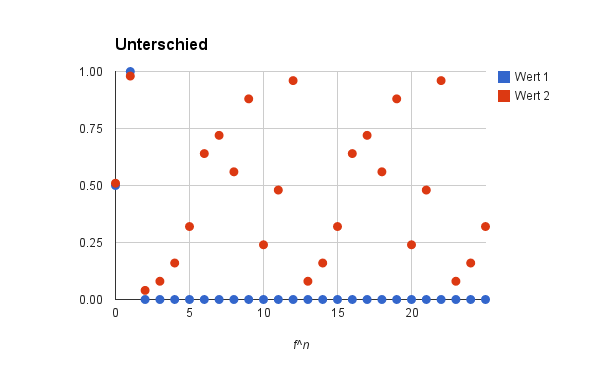
\includegraphics[scale=0.5]{bilder/Unterschied}
\end{figure}

Zunächst verdoppelte sich der Fehler, dann  





\end{document}